\documentclass[11pt]{article}
% generated by Madoko, version 1.2.3
%mdk-data-line={1}


\usepackage[heading-base={2},section-num={False},bib-label={hide},fontspec={True}]{madoko2}
\usepackage[top=1in, bottom=1.25in, left=1in, right=1in]{geometry}
\usepackage{fancyhdr}
\usepackage{mathpartir}
\usepackage{amscd}
\usepackage[version=3]{mhchem}
%mdk-data-line={18}

  \setlength{\headheight}{30pt}
  \renewcommand{\footrulewidth}{0.5pt}

\begin{document}



{\mdfontfamily{UtopiaStd-Regular}
%mdk-data-line={148}
\mdxtitleblockstart{}
%mdk-data-line={148}
\mdxtitle{{\sffamily{\bfseries\mdline{148}Petr4 Type System Formalization}}}%mdk
\mdxauthorstart{}
%mdk-data-line={153}
\mdxauthorname{\mdline{153}Parisa Ataei, Ryan Doenges, Nate Foster}%mdk

%mdk-data-line={156}
\mdxauthoraddress{\mdline{156}Cornell University}%mdk
\mdxauthorend
%mdk-data-line={165}
\mdxtitlefooter{{\sffamily{\bfseries\mdline{165}2022-05-16}}}%mdk
\mdtitleauthorrunning{}{}\mdxtitleblockend%mdk
%mdk-begin-texraw
%mdk-data-line={151}
\mdDefineUnicode{10214}{\ensuremath{\llbracket}}
\mdDefineUnicode{10215}{\ensuremath{\rrbracket}}

%mdk-data-line={155}
\begin{abstract}%mdk

%mdk-data-line={156}
\noindent\mdline{156}P4 is a language for programming the data plane of network
devices. Petr4 provides a clean-slate definitional interpreter
and a core calculus that models a fragment of P4. This document
provides a definition of Petr4\mdline{159}'\mdline{159}s type system that is consistent
with its implementation. The target audience of this document
includes developers and debuggers who work on P4 implementations
such as Petr4 and P4C. In essence, this document may be of
interest to programmers who are interested in understanding
the implementation of Petr4 deeply.%mdk
%mdk
\end{abstract}%mdk
%mdk-data-line={168;ops.tex:1}
%stuff here and there:
\renewcommand{\or}{\ | \ }
\newcommand{\whereBulletIs}{,\textit{ where } \bullet \textit{ is }}
\newcommand{\whereIs}[1]{,\textit{ where } {#1} \textit{ is }}
\newcommand{\where}[1]{,\textit{ where } {#1}}
\newcommand{\textOr}{\textit{ or }}
\newcommand{\numeric}[1]{\mathit{numeric}({#1})}
\newcommand{\error}{\mathit{error}}
\newcommand{\cond}{\mathit{cond}}
\newcommand{\prim}[1]{{#1}^\prime}
\newcommand{\pprim}[1]{{#1}^{\prime\prime}}
\newcommand{\so}[2]{{#1} \Rightarrow {#2}}
\newcommand{\lookupEnv}[1]{\env({#1})}
\newcommand{\emp}{[\ ]}

% separator
\newcommand{\rn}[1]{\TirName{#1}}
\newcommand{\rSep}{\rn{-}}

\newcommand*{\rE}{\rSep\rn{E}}
\newcommand*{\restJ}{\rn{Rest}}

%typing judgments:
\newcommand{\envOne}[2]{\Delta, T, \Gamma \vdash {#1} : {#2}}
\newcommand{\expenv}[4]{\env, \ctxt \vdash {#1} \leadsto {#2}, {#3}, {#4}}
\newcommand{\expenvWithCtxt}[5]{\env, {#1} \vdash {#2} \leadsto {#3}, {#4}, {#5}}
\newcommand{\coerceBinArgsEnv}[3]{\env, \ctxt \vdash {#1} \twoheadrightarrow ({#2}; {#3})}
\newcommand{\binOpEnv}[4]{\env \vdash {#1} \hookrightarrow {#2}, {#3}, {#4}}
\newcommand{\typWellFormed}[1]{\env \vdash {#1}}

%contexts:
\newcommand{\cte}{\mathit{CONSTANT}}

%operators:
\newcommand{\mask}[2]{{#1} \&\&\& {#2}}
\newcommand{\range}[2]{{#1}..{#2}}
\newcommand{\ternary}[3]{{#1} ? {#2} : {#3}}
\newcommand{\errMem}[1]{\mathit{error}.{#1}}
\newcommand{\typMem}[2]{{#1}.{#2}}
\newcommand{\shiftR}{\gg}
\newcommand{\shiftL}{\ll}
\newcommand{\concat}{+\!+\ }
\newcommand{\restOps}{\odot}
\newcommand{\ops}{\odot}
\newcommand{\cast}[2]{({#1}){#2}}
\newcommand{\plusSat}{\vert+\vert}
\newcommand{\subSat}{\vert-\vert}
\newcommand{\bitAnd}{\&}
\newcommand{\bitOr}{\vert}
\newcommand{\bitXor}{\hat{}}
\newcommand{\bitComplement}{\sim}
\renewcommand{\div}{/}
\renewcommand{\mod}{\%}

%metavariables:
\newcommand{\env}{e}
\newcommand{\typ}{t}
\newcommand{\ctxt}{c}
\newcommand{\bool}{b}
\newcommand{\str}{s}
\newcommand{\width}{w}
\newcommand{\val}{v}
\newcommand{\bit}{\mathit{bit}}
\renewcommand{\int}{n}
\newcommand{\bitWidth}[2]{{#1}_{#2}}
\newcommand{\intWidth}[2]{{#1}_{#2}}
\newcommand{\name}{\mathit{name}}
\renewcommand{\array}{a}
\renewcommand{\index}{i}
\newcommand{\arrayAccess}[2]{{#1}[{#2}]}
\newcommand{\size}{n}
\newcommand{\high}{h}
\newcommand{\low}{l}
\newcommand{\bitString}{bs}
\newcommand{\bitStringAccess}[3]{{#1}[{#2}:{#3}]}
\renewcommand{\exp}{\mathit{exp}}
\newcommand{\field}{f}
\renewcommand{\arg}{\mathit{arg}}


%function helpers
\newcommand{\isNumeric}[1]{\mathit{is\_numeric}({#1})}
\newcommand{\isArray}[1]{\mathit{is\_array}({#1})}
\newcommand{\compileTimeEval}[1]{\llbracket{#1}\rrbracket_\env}
\newcommand{\implicitCast}[2]{\mathit{implicit\_cast}({#1},{#2})_\env}
\newcommand{\reduceEnums}[1]{\mathit{reduce\_enums}({#1}.\typ)_\env} 
\newcommand{\inOrLess}[2]{\mathit{in\_or\_directionless}({#1},{#2})}
\newcommand{\typEq}[3]{{#2} ==_{\env,{#1}} {#3}}
\newcommand{\typHasEq}[1]{\mathit{has\_equality}({#1})_\env}
\newcommand{\nonNeg}[1]{\mathit{is\_nonneg\_numeric}({#1})_\env}
\newcommand{\pos}[1]{\mathit{is\_pos\_numeric}({#1})_\env}
\newcommand{\compTimeKnown}[1]{\mathit{compile\_time\_known}({#1})_\env}
\newcommand{\sat}[1]{\mathit{saturate}({#1})_\env}
\newcommand{\trans}[2]{\mathit{translate}({#1})_{\env,{#2}}}
\newcommand{\isValidNestedTyp}[2]{\mathit{is\_valid\_nested\_type}({#1},{#2})_\env}
%{#1} is outer, 2 is inner
\newcommand{\noDup}[1]{\mathit{no\_duplicate}({#1})}
\newcommand{\explicitCastOK}[2]{\mathit{explicit\_cast\_ok} ({#1}, {#2})_\env}

%types:
\newcommand{\bitWidthTyp}[1]{\mathit{bit}<\!{#1}\!>}
\newcommand{\intWidthTyp}[1]{\mathit{int}<\!{#1}\!>}
\newcommand{\boolTyp}{\mathit{bool}}
\newcommand{\stringTyp}{\mathit{string}}
\newcommand{\integerTyp}{\mathit{integer}}
\newcommand{\bitStringTyp}[2]{\mathit{bit[{#1}-{#2}]}}
\newcommand{\intTyp}{\mathit{int}}
\newcommand{\setTyp}[1]{\mathit{set}<\!{#1}\!>}
\newcommand{\errTyp}{\mathit{error}}
\newcommand{\varBitTyp}[1]{\mathit{varbit}<{#1}>}
\newcommand{\matchKindTyp}{\mathit{match\_kind}}
\newcommand{\voidTyp}{\mathit{void}}
\newcommand{\arrayTyp}[2]{{#1}[{#2}]}
\newcommand{\tupleTyp}[2]{<{#1},\ldots,{#2}>}
\newcommand{\listTyp}[2]{[{#1},\ldots,{#2}]}
\newcommand{\enumTyp}{\mathit{enum}\ {\typ}\ {\name}\{\name_1,\ldots,\name_n\}}
\newcommand{\enumTypNoTyp}{\mathit{enum} \ {\name}\{\name_1,\ldots,\name_n\}}
\newcommand{\recordTyp}{\mathit{record}\{\field_1:\typ_1,\ldots,\field_n:\typ_n \}}
\newcommand{\headerUnionTyp}{\mathit{header\_union}\{\field_1:\typ_1,\ldots,\field_n:\typ_n \}}
\newcommand{\headerTyp}{\mathit{header}\{\field_1:\typ_1,\ldots,\field_n:\typ_n \}}
\newcommand{\structTyp}{\mathit{struct}\{\field_1:\typ_1,\ldots,\field_n:\typ_n \}}
\newcommand{\newTypeTyp}[2]{\mathit{type}\ {#1}\ {#2}}

%directions:
\newcommand{\less}{\mathit{directionless}}
\newcommand{\dir}{d}
\renewcommand{\in}{\mathit{in}}
\newcommand{\out}{\mathit{out}}

\mdline{171}
\begin{mdtoc}%mdk

\section*{Contents}\mdlabel{sec-contents}{2}%mdk%mdk

\begin{mdtocblock}%mdk

\mdtocitemx{sec-overview}{\mdref{sec-overview}{1.\hspace*{0.5em}Overview}}%mdk

\begin{mdtocblock}%mdk

\mdtocitemx{sec-conn}{\mdref{sec-conn}{1.1.\hspace*{0.5em}Connecting To The Implementation}}%mdk

\mdtocitemx{sec-arch}{\mdref{sec-arch}{1.2.\hspace*{0.5em}Architecture}}%mdk
%mdk
\end{mdtocblock}%mdk

\mdtocitemx{sec-type-system}{\mdref{sec-type-system}{2.\hspace*{0.5em}Type System}}%mdk

\begin{mdtocblock}%mdk

\mdtocitemx{sec-expressions-typing-rules}{\mdref{sec-expressions-typing-rules}{2.1.\hspace*{0.5em}Expression's Typing Rules}}%mdk

\begin{mdtocblock}%mdk

\mdtocitemx{sec-coerce-binary-operation-arguments-auxiliary-judgment}{\mdref{sec-coerce-binary-operation-arguments-auxiliary-judgment}{2.1.1.\hspace*{0.5em}Coerce Binary Operation Arguments Auxiliary Judgment}}%mdk

\mdtocitemx{sec-check-binary-operation-auxiliary-judgment}{\mdref{sec-check-binary-operation-auxiliary-judgment}{2.1.2.\hspace*{0.5em}Check Binary Operation Auxiliary Judgment}}%mdk

\mdtocitemx{sec-type-well-formed-auxiliary-judgment}{\mdref{sec-type-well-formed-auxiliary-judgment}{2.1.3.\hspace*{0.5em}Type Well-Formed Auxiliary Judgment}}%mdk
%mdk
\end{mdtocblock}%mdk
%mdk
\end{mdtocblock}%mdk
%mdk
\end{mdtocblock}%mdk
%mdk
\end{mdtoc}%mdk

%mdk-data-line={173}
\section{\mdline{173}1.\hspace*{0.5em}\mdline{173}Overview}\mdlabel{sec-overview}{1}%mdk%mdk

%mdk-data-line={175}
\noindent\mdline{175}This document defines the type system of Petr4. The type system
conducts three tasks simultaneously:%mdk

%mdk-data-line={178}
\begin{enumerate}[noitemsep,topsep=\mdcompacttopsep]%mdk

%mdk-data-line={178}
\item\mdline{178}It type checks P4 programs.%mdk

%mdk-data-line={179}
\item\mdline{179}It conducts type inference.%mdk

%mdk-data-line={180}
\item\mdline{180}It does a pass from the surface syntax to the first IR.%mdk
%mdk
\end{enumerate}%mdk

%mdk-data-line={183}
\subsection{\mdline{183}1.1.\hspace*{0.5em}\mdline{183}Connecting To The Implementation}\mdlabel{sec-conn}{1.1}%mdk%mdk

%mdk-data-line={185}
\noindent\mdline{185}The following locates each data type in the implementation
(\mdline{186}\href{https://github.com/verified-network-toolchain/petr4}{{\ttfamily https://\hspace{0pt}github.\hspace{0pt}com/\hspace{0pt}verified-\hspace{0pt}network-\hspace{0pt}toolchain/\hspace{0pt}petr4}}\mdline{186}):%mdk

%mdk-data-line={188}
\begin{itemize}[noitemsep,topsep=\mdcompacttopsep]%mdk

%mdk-data-line={188}
\item\mdline{188}The surface AST is \mdline{188}\emph{types.program}\mdline{188}%mdk

%mdk-data-line={189}
\item\mdline{189}The type of programs of the surface syntax is \mdline{189}\emph{types.type.t}\mdline{189}%mdk

%mdk-data-line={190}
\item\mdline{190}The first IR is \mdline{190}\emph{prog.program}\mdline{190}%mdk

%mdk-data-line={191}
\item\mdline{191}The type of the first IR is \mdline{191}\emph{prog.type.t}\mdline{191}%mdk
%mdk
\end{itemize}%mdk

%mdk-data-line={193}
\noindent\mdline{193}For simplicity, we have removed the information that is needed to report when an error
happens. Such information is passed around in the surface syntax as a field (called
\mdline{195}\mdcode{{\mdfontfamily{LuxiMono}{\mdfontsize{\dimfont{0.75}}tags}}}\mdline{195}) of record for all data types.%mdk

%mdk-data-line={197}
\subsection{\mdline{197}1.2.\hspace*{0.5em}\mdline{197}Architecture}\mdlabel{sec-arch}{1.2}%mdk%mdk

%mdk-data-line={199}
\noindent\mdline{199}Figure\mdline{199}~\mdref{fig-arch}{\mdcaptionlabel{1}}\mdline{199} depicts part of Petr4\mdline{199}'\mdline{199}s architecture that contains the type system.
After lexing and parsing a P4 program we get a program in our surface syntax. This
program is then passed through the \mdline{201}\emph{elaborator}\mdline{201} where type variables are introduced
instead of underscore and new type variable names are generated for variables with the
same name but in different scopes. This document does not discuss the innerworkings of
\mdline{204}\mdcode{{\mdfontfamily{LuxiMono}{\mdfontsize{\dimfont{0.75}}elaborate}}}\mdline{204}. Then, the program is passed through the type system (encoded in \mdline{204}\mdcode{{\mdfontfamily{LuxiMono}{\mdfontsize{\dimfont{0.75}}checker}}}\mdline{204}).
This document discusses the innerworking of the type system extensively. Finally, the
program is evaluated.%mdk

%mdk-data-line={208}
\begin{figure}[tbp]%mdk
\begin{mdcenter}%mdk

%mdk-data-line={209}
\noindent\mdline{209}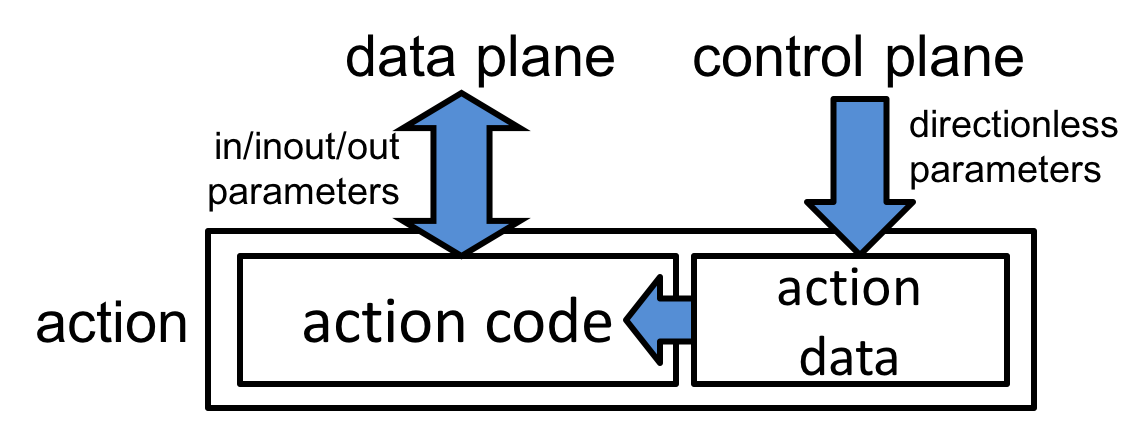
\includegraphics[keepaspectratio=true,width=\dimwidth{1.00}]{figs/petr4/arch}{}\mdline{209}%mdk

%mdk-data-line={210}
\mdhr{}%mdk

%mdk-data-line={211}
\noindent\mdline{211}\mdcaption{\textbf{Figure~\mdcaptionlabel{1}.}~\mdcaptiontext{Part of Petr4's achitecture.}}%mdk
%mdk
\end{mdcenter}\mdlabel{fig-arch}{1}%mdk
%mdk
\end{figure}%mdk

%mdk-data-line={213}
\section{\mdline{213}2.\hspace*{0.5em}\mdline{213}Type System}\mdlabel{sec-type-system}{2}%mdk%mdk

%mdk-data-line={215}
\noindent\mdline{215}some general explanation of the type system and the judgments.%mdk

%mdk-data-line={217}
\subsection{\mdline{217}2.1.\hspace*{0.5em}\mdline{217}Expression\mdline{217}'\mdline{217}s Typing Rules}\mdlabel{sec-expressions-typing-rules}{2.1}%mdk%mdk

%mdk-data-line={218}
\noindent\mdline{218}translate typ translate a surface type to the IR\mdline{218}'\mdline{218}s type. we don\mdline{218}'\mdline{218}t present these types
since their difference isn\mdline{219}'\mdline{219}t much.
saturate typ saturates a type. Eliminate all type references in typ and replace them with the type they refer to. The result of saturation will contain no TypeName constructors anywhere. It may contain TypeName constructors.
e(name) looks up name in the environment and returns its type and direction.
is array determines whether a type is an array type.
is numberic determines whether a type is numeric.
compile time evaluation evaluates the expression expr at compile time.
explicit cast ok checks whether typ1 can be converted to typ2 under e based on P4\mdline{225}'\mdline{225}s specification of 8.9.1. Explicit casts.%mdk

%mdk-data-line={227}
\begin{mdbpadding}{1ex}%mdk
\begin{mdcenter}%mdk

%mdk-data-line={228}
%mdk-data-line={229}
\begin{mathpar}
  \small

  \inferrule[Bool]
     {}
     {\expenv \bool \bool \boolTyp \less}

  \inferrule[String]
     {}
     {\expenv \str \str \stringTyp \less}

  \inferrule[Integer]
     {}
     {\expenv \int \int \integerTyp \less}

  \inferrule[Bit]
     {}
     {\expenv {\bitWidth \bit \width} {\bitWidth \bit \width} {\bitWidthTyp \width} \less}

  \inferrule[Int]
     {  }
     {\expenv {\intWidth \int \width} {\intWidth \int \width} {\intWidthTyp \width} {\less}}

  \inferrule[Name]
     {\lookupEnv \name = (\typ, \dir)}
     {\expenv \name \name \typ \dir}

  \inferrule[ArrayAccess]
     {\expenv {\array} {\prim \array} {\arrayTyp \typ \size} \dir \\
      \expenv \index {\prim \index} {\prim \typ} {\prim \dir} \\
      \isArray {\arrayTyp \typ \size} \\
      \isNumeric {\prim \typ}}
     {\expenv {\arrayAccess \array \index} {\arrayAccess {\prim \array} {\prim \index}} \typ \dir }

  \inferrule[BitStringAccess]
     {\expenvWithCtxt \cte \high {\prim \high} {\typ_\high} {\dir_\high} \\
      \isNumeric {\typ_\high} \\
      \pprim \high = \compileTimeEval {\prim \high} \\
      \expenvWithCtxt \cte \low {\prim \low} {\typ_\low} {\dir_\low} \\
      \isNumeric {\typ_\low} \\
      \pprim \low = \compileTimeEval {\prim \low} \\
      0 \leq \pprim \low < \width \\
      \pprim l \leq \pprim h < \width \\
      \expenv \bitString {\prim \bitString} \typ \dir \\
      \typ = \intWidthTyp \width \textOr \bitWidthTyp \width}
     {\expenv {\bitStringAccess \bitString \low \high} {\bitStringAccess \bitString {\pprim \low} {\pprim \high}} {\bitStringTyp {\pprim \low} {\pprim \high}} \dir }

  \inferrule[List]
     {1 \leq i \leq n; \expenv {\exp_i} {\prim {\exp_i}} {\typ_i} {\dir_i}}
     {\expenv {[\exp_1, \ldots, \exp_n]} {[\exp_1, \ldots, \exp_n]} {[\typ_1, \ldots, \typ_n]} \less }

  \inferrule[Record]
     {1 \leq i \leq n; \expenv {\exp_i} {\prim {\exp_i}} {\typ_i} {\dir_i}  }
     {\expenv {\{\field_1 = \exp_1, \ldots, \field_n = \exp_n \}} {\{\field_1 = \prim {\exp_1}, \ldots, \field_n = \prim {\exp_n} \}} {\{\field_1 : \typ_1, \ldots, \field_n : \typ_n \}} \less  }

  \inferrule[LogicalNegation]
     { \expenv \exp {\prim \exp} \boolTyp \dir }
     { \expenv {!\exp} {!\prim \exp} \boolTyp \dir }

  \inferrule[BitwiseComplement]
     { \expenv \exp {\prim \exp} {\bitWidthTyp \width} \dir }
     { \expenv {\bitComplement\!\exp} {\bitComplement\!\prim \exp} {\bitWidthTyp \width} \dir }

  \inferrule[UnaryMinusCTK]
     { \expenv \exp {\prim \exp} \intTyp \dir }
     { \expenv {-\exp} {-\prim \exp} \intTyp \dir }

  \inferrule[UnaryMinus]
     { \expenv \exp {\prim \exp} {\intWidthTyp \width} \dir }
     { \expenv {-\exp} {-\prim \exp} {\intWidthTyp \width} \dir }

  \inferrule[BinaryOps]
     {\coerceBinArgsEnv {\exp_1 \oplus \exp_2} {\prim {\exp_1}} {\prim {\exp_2}} \\
      \binOpEnv {\prim {\exp_1} \oplus \prim {\exp_2}} {\pprim {\exp_1} \oplus \pprim {\exp_2}} \typ \dir }
     { \expenv {\exp_1 \oplus \exp_2} {\prim {\exp_1} \oplus \prim {\exp_2}} \typ \dir }

\end{mathpar}%mdk
%mdk
\end{mdcenter}%mdk
\end{mdbpadding}%mdk

%mdk-data-line={309}
\begin{mdbpadding}{1ex}%mdk
\begin{mdcenter}%mdk

%mdk-data-line={310}
%mdk-data-line={311}
\begin{mathpar}
  \small

  \inferrule[Cast]
     { \expenv \exp {\exp_1} {\typ_1} \dir \\
       \typ_2 = \sat {\typ_1} \\
       \typ_3 = \trans {\typ_2} {\emp} \\
       \typ_4 = \sat {\typ_3} \\
       \typWellFormed {\typ_3} \\
       \explicitCastOK {\typ_1} {\typ_3}}
     { \expenv {\cast \typ \exp} {\cast {\typ_1} {\exp_1}} {\typ_3} \less  }

  \inferrule[TypeMember]
     {\lookupEnv {\typMem \typ \name} = (\typ, \dir)  }
     {\expenv {\typMem \typ \name} {\typMem \typ \name} \typ \less  }

  \inferrule[ErrorMember]
     {\lookupEnv {\errMem \name} = (\errTyp, \dir)  }
     {\expenv {\errMem \name} {\errMem \name} \errTyp \less  }

  \inferrule[ExpressionMember]
     { blah }
     { blah}

  \inferrule[Ternary]
     {\expenv {\exp_1} {\prim {\exp_1}} \boolTyp {\dir_1} \\
      \expenv {\exp_2} {\prim {\exp_2}} {\typ_1} {\dir_2} \\
      \expenv {\exp_3} {\prim {\exp_3}} {\typ_2} {\dir_3}\\
      \typ_1 = \typ_2 \\
      \typ_1 \neq \integerTyp}
     {\expenv {\ternary {\exp_1} {\exp_2} {\exp_3}} {\ternary {\prim {\exp_1}} {\prim {\exp_2}} {\prim {\exp_3}}} {\typ_1} \less }

  \inferrule[FunctionCall]
     { blah }
     { blah }
     % { \expenv {\exp (\typ_1 \arg_1, \ldots, \typ_n \arg_n)}  }

% function type: <return type> <function name>(x1,...,xn) {...}

  \inferrule[NamelessIinstantiation]
     { blah }
     { blah }

  \inferrule[Mask]
     {\expenv {\exp_1} {\prim {\exp_1}} {\typ_1} {\dir_1} \\
      \expenv {\exp_2} {\prim {\exp_2}} {\typ_2} {\dir_2} \\
      \left( \so {\typ_1 = \typ_2 = \bitWidthTyp \width} {\typ = \bitWidthTyp \width}\right) \\
      \textOr
      \left( \so {\typ_1 = \typ_2 = \integerTyp} {\typ = \integerTyp}\right) \\
      \textOr
      \left( \so {\typ_1 = \bitWidthTyp \width, \typ_2 = \integerTyp} {\typ = \bitWidthTyp \width}\right) \\
      \textOr
      \left( \so {\typ_1 = \integerTyp, \typ_2 = \bitWidthTyp \width} {\typ = \bitWidthTyp \width}\right)
      }
     {\expenv {\mask {\exp_1} {\exp_2}} {\mask {\prim \exp_1} {\prim \exp_2}} {\setTyp \typ} \less  }

  \inferrule[Range]
     { \expenv \low {\prim \low} \typ {\dir_\low} \\
       \expenv \high {\prim \high} \typ {\dir_\high} \\
       \typ_\low = \typ_\high = \bitWidthTyp \width \textOr \intWidthTyp \width \textOr \integerTyp}
     { \expenv {\range \low \high} {\range {\prim \low} {\prim \high}} {\setTyp \typ} \dir }


\end{mathpar}%mdk
%mdk
\end{mdcenter}%mdk
\end{mdbpadding}%mdk

%mdk-data-line={378}
\subsubsection{\mdline{378}2.1.1.\hspace*{0.5em}\mdline{378}Coerce Binary Operation Arguments Auxiliary Judgment}\mdlabel{sec-coerce-binary-operation-arguments-auxiliary-judgment}{2.1.1}%mdk%mdk

%mdk-data-line={379}
\noindent\mdline{379}Let implicitCast typ1 typ2 be defined as follows to describe P4\mdline{379}'\mdline{379}s implicit
casting behavior on operands in binary expressions:
      \mdline{381}\mdbr
\mdline{382}cast typ exp produces a cast expression if the type of exp is different from the
type typ.%mdk

%mdk-data-line={385}
\mdline{385}The restJ rule stands for all other binary operations.%mdk

%mdk-data-line={387}
\begin{mdbpadding}{1ex}%mdk
\begin{mdcenter}%mdk

%mdk-data-line={388}
%mdk-data-line={389}
\begin{mathpar}
  \small

  \inferrule[ShiftRight]
     { \expenv {\exp_1} {\prim {\exp_1}} {\typ_1} {\dir_1} \\
       \expenv {\exp_2} {\prim {\exp_2}} {\typ_2} {\dir_2}}
     { \coerceBinArgsEnv {\exp_1 \shiftR \exp_2} {\prim {\exp_1}, {\typ_1}, {\dir_1}} {\prim {\exp_2}, {\typ_2}, {\dir_2}}  }

  \inferrule[ShiftLeft]
     { \expenv {\exp_1} {\prim {\exp_1}} {\typ_1} {\dir_1} \\
       \expenv {\exp_2} {\prim {\exp_2}} {\typ_2} {\dir_2}}
     { \coerceBinArgsEnv {\exp_1 \shiftL \exp_2} {\prim {\exp_1}} {\prim {\exp_2}} {\prim {\exp_1}, {\typ_1}, {\dir_1}} {\prim {\exp_2}, {\typ_2}, {\dir_2}} }

  \inferrule[BitConcatenation]
     { \expenv {\exp_1} {\prim {\exp_1}} {\typ_1} {\dir_1} \\
       \expenv {\exp_2} {\prim {\exp_2}} {\typ_2} {\dir_2}}
     { \coerceBinArgsEnv {\exp_1 \concat \exp_2} {\prim {\exp_1}, {\typ_1}, {\dir_1}} {\prim {\exp_2}, {\typ_2}, {\dir_2}} }

  \inferrule[Rest]
     { \expenv  {\exp_1} {\prim {\exp_1}} {\typ_1} {\dir_1} \\
       \expenv {\exp_2} {\prim {\exp_2}} {\typ_2} {\dir_2} \\
       t = \implicitCast {\typ_1} {\typ_2} \\
       {\pprim {\exp_1}} = \cast \typ {\prim {\exp_1}}, {\typ_1}, {\dir_1} \\
       {\pprim {\exp_2}} = \cast \typ {\prim {\exp_2}}, {\typ_2}, {\dir_2}}
     { \coerceBinArgsEnv {\exp_1 \restOps \exp_2} {\pprim {\exp_1}} {\pprim {\exp_2}} }

\end{mathpar}%mdk
%mdk
\end{mdcenter}%mdk
\end{mdbpadding}%mdk

%mdk-data-line={419}
\subsubsection{\mdline{419}2.1.2.\hspace*{0.5em}\mdline{419}Check Binary Operation Auxiliary Judgment}\mdlabel{sec-check-binary-operation-auxiliary-judgment}{2.1.2}%mdk%mdk

%mdk-data-line={420}
\noindent\mdline{420}reduce enums removes all the enums recursively after reducing a type.
in\mdline{421}\_\mdline{421}or\mdline{421}\_\mdline{421}dirless(typ1, typ2) retunrs direction of In if both typ1 and typ2 have In direction, o.w., it returns a directionless direction. 
is true if and only if expression type t1 is equivalent to expression type t2 under environment env. Alpha equivalent types are equal. it takes the list of variables of the two types.
is nonneg and is pos evaluate an expression at compile time and check if it\mdline{423}'\mdline{423}s a nonneg or pos numeric.
compile time known determinez if the value of an expression can be known at compile time.
   it returns true for externs, packages, controls, and parsers..%mdk

%mdk-data-line={427}
\begin{mdbpadding}{1ex}%mdk
\begin{mdcenter}%mdk

%mdk-data-line={428}
%mdk-data-line={429}
\begin{mathpar}
  \small

  \inferrule[LogicalOps($\ops=\&,\vert$)]
     { \typ_1 = \reduceEnums {\exp_1} \\
       \typ_2 = \reduceEnums {\exp_2} \\
       \dir = \inOrLess {\typ_1} {\typ_2} \\
       \typ_1 = \typ_2 = \boolTyp}
     { \binOpEnv {\exp_1 \restOps \exp_2} {\exp_1 \restOps \exp_2} \boolTyp \dir }

  \inferrule[NumericOps($+, -, *$)]
     { \typ_1 = \reduceEnums {\exp_1} \\
       \typ_2 = \reduceEnums {\exp_2} \\
       \dir = \inOrLess {\typ_1} {\typ_2} \\
       \typ_1 = \typ_2 = \bitWidthTyp \width \textOr \integerTyp \textOr \intWidthTyp \width }
     { \binOpEnv {\exp_1 \restOps \exp_2} {\exp_1 \restOps \exp_2} {\typ_1} \dir }

  \inferrule[EqualityChecks($==, !=$)]
     { \typ_1 = \reduceEnums {\exp_1} \\
       \typ_2 = \reduceEnums {\exp_2} \\
       \typEq {\emp} {\typ_1} {\typ_2} \\
       \typHasEq {\typ_1} }
     { \binOpEnv {\exp_1 \restOps \exp_2} {\exp_1 \restOps \exp_2} \boolTyp \dir }

  \inferrule[OpSat($\plusSat,\subSat$)]
     { \typ_1 = \reduceEnums {\exp_1} \\
       \typ_2 = \reduceEnums {\exp_2} \\
       \dir = \inOrLess {\typ_1} {\typ_2} \\
       \typ_1 = \typ_2 = \bitWidthTyp \width \textOr \intWidthTyp \width}
     { \binOpEnv {\exp_1 \restOps \exp_2} {\exp_1 \restOps \exp_2} {\typ_1} \dir }

  \inferrule[BitwiseOps($\bitAnd, \bitOr, \bitXor, \bitComplement$)]
     { \typ_1 = \reduceEnums {\exp_1} \\
       \typ_2 = \reduceEnums {\exp_2} \\
       \dir = \inOrLess {\typ_1} {\typ_2} \\
       \typ_1 = \typ_2 = \bitWidthTyp \width \textOr \intWidthTyp \width}
     { \binOpEnv {\exp_1 \restOps \exp_2} {\exp_1 \restOps \exp_2} {\typ_1} \dir }

  \inferrule[BitstringConcatenation]
     { \typ_1 = \reduceEnums {\exp_1} \\
       \typ_2 = \reduceEnums {\exp_2} \\
       \dir = \inOrLess {\typ_1} {\typ_2} \\
       \left( \so {\typ_1 = \bitWidthTyp {\width_1}, \typ_2 = \bitWidthTyp {\width_2} \textOr \intWidthTyp {\width_2}} {\typ = \bitWidthTyp {\width_1 + \width_2}} \right) \\
       \textOr \left( \so {\typ_1 = \intWidthTyp {\width_1}, \typ_2 = \bitWidthTyp {\width_2} \textOr \intWidthTyp {\width_2}} {\typ = \intWidthTyp {\width_1 + \width_2}} \right) }
     { \binOpEnv {\exp_1 \concat \exp_2} {\exp_1 \concat \exp_2} {\typ} \dir }

  \inferrule[ComparisonOps($<, \leq, >, \geq$)]
     { \typ_1 = \reduceEnums {\exp_1} \\
       \typ_2 = \reduceEnums {\exp_2} \\
       \dir = \inOrLess {\typ_1} {\typ_2} \\
       \left( \typ_1 = \typ_2 = \integerTyp \right) \\
       \textOr \left( \typ_1 = \typ_2 = \bitWidthTyp \width \right) \\
       \textOr \left( \typ_1 = \typ_2 = \intWidthTyp \width \right)}
     { \binOpEnv {\exp_1 \restOps \exp_2} {\exp_1 \restOps \exp_2} \boolTyp \dir }

  \inferrule[DivOps($\div, \mod$)]
     { \typ_1 = \reduceEnums {\exp_1} \\
       \typ_2 = \reduceEnums {\exp_2} \\
       \dir = \inOrLess {\typ_1} {\typ_2} \\
       \left( \so {\typ_1 = \typ_2 = \integerTyp, \nonNeg {\exp_1}, \pos {\exp_2}}  {\typ = \integerTyp} \right) \\
       \textOr \left( \so {\typ_1 = \typ_2 = \bitWidthTyp \width, \nonNeg {\exp_1}, \pos {\exp_2}}  {\typ = \bitWidthTyp \width} \right) }
     { \binOpEnv {\exp_1 \restOps \exp_2} {\exp_1 \restOps \exp_2} \typ \dir }

  \inferrule[ShiftOps($\shiftL,\shiftR$)]
     { \typ_1 = \reduceEnums {\exp_1} \\
       \typ_2 = \reduceEnums {\exp_2} \\
       \dir = \inOrLess {\typ_1} {\typ_2} \\
       \nonNeg {\exp_2} \\
       \left( \typ_1 = \bitWidthTyp \width \textOr \intWidthTyp \width \right) \\
       \textOr \left( \typ_1 = \integerTyp, \compTimeKnown {\exp_2} \right) }
     { \binOpEnv {\exp_1 \restOps \exp_2} {\exp_1 \restOps \exp_2} {\typ_1} \dir }

\end{mathpar}%mdk
%mdk
\end{mdcenter}%mdk
\end{mdbpadding}%mdk

%mdk-data-line={505}
\subsubsection{\mdline{505}2.1.3.\hspace*{0.5em}\mdline{505}Type Well-Formed Auxiliary Judgment}\mdlabel{sec-type-well-formed-auxiliary-judgment}{2.1.3}%mdk%mdk

%mdk-data-line={506}
\noindent\mdline{506}it saturates all types first and then checks well-formedness. for breviety, we don\mdline{506}'\mdline{506}t
include the saturation in rules.
is valid nested type outer inner checks whether the nested type is taking valid types in its inner and outer type based on P4\mdline{508}'\mdline{508}s description of type nesting rules section 7.2.7 (provide link). 
no duplicate determines if there are duplicate fields in a structure/type.%mdk

%mdk-data-line={510}
\begin{mdbpadding}{1ex}%mdk
\begin{mdcenter}%mdk

%mdk-data-line={511}
%mdk-data-line={512}
\begin{mathpar}
  \small

  \inferrule[Bool]
     { }
     { \typWellFormed \boolTyp }

  \inferrule[String]
     { }
     { \typWellFormed \stringTyp }

  \inferrule[Integer]
     { }
     { \typWellFormed \integerTyp }

  \inferrule[Int]
     { }
     { \typWellFormed {\intWidthTyp \width} }

  \inferrule[Bit]
     { }
     { \typWellFormed {\bitWidthTyp \width} }

  \inferrule[VarBit]
     { }
     { \typWellFormed {\varBitTyp \width} }

  \inferrule[Error]
     { }
     { \typWellFormed \errTyp}

  \inferrule[Void]
     { }
     { \typWellFormed \voidTyp}

  \inferrule[MatchKind]
     { }
     { \typWellFormed \matchKindTyp}

  \inferrule[Array]
     { \typWellFormed \typ \\
       \isValidNestedTyp {\arrayTyp \typ \size} {\typ}}
     { \typWellFormed {\arrayTyp \typ \size} }

  \inferrule[Tuple]
     { 1 \leq i \leq; \typWellFormed {\typ_i} \\
       1 \leq i \leq; \isValidNestedTyp {\tupleTyp {\typ_1} {\typ_n}} {\typ_i}}
     { \typWellFormed {\tupleTyp {\typ_1} {\typ_n}} }

  \inferrule[List]
     { 1 \leq i \leq; \typWellFormed {\typ_i} \\
       1 \leq i \leq; \isValidNestedTyp {\listTyp {\typ_1} {\typ_n}} {\typ_i}}
     { \typWellFormed {\listTyp {\typ_1} {\typ_n}} }

  \inferrule[Set]
     { \typWellFormed \typ }
     { \typWellFormed {\setTyp \typ} }

  \inferrule[EnumWithType]
     { \typWellFormed \typ }
     { \typWellFormed \enumTyp }

  \inferrule[EnumWithoutType]
     {  }
     { \typWellFormed \enumTypNoTyp }

  \inferrule[Record]
     { 1 \leq i \leq; \typWellFormed {\typ_i} \\
       1 \leq i \leq; \isValidNestedTyp \recordTyp {\typ_i} \\
       \noDup {\field_1, \ldots, \field_n}}
     { \typWellFormed \recordTyp }

  \inferrule[HeaderUnion]
     { 1 \leq i \leq; \typWellFormed {\typ_i} \\
       1 \leq i \leq; \isValidNestedTyp \headerUnionTyp {\typ_i} \\
       \noDup {\field_1, \ldots, \field_n}}
     { \typWellFormed \headerUnionTyp }

  \inferrule[Struct]
     { 1 \leq i \leq; \typWellFormed {\typ_i} \\
       1 \leq i \leq; \isValidNestedTyp \structTyp {\typ_i} \\
       \noDup {\field_1, \ldots, \field_n}}
     { \typWellFormed \structTyp }

  \inferrule[Header]
     { 1 \leq i \leq; \typWellFormed {\typ_i} \\
       1 \leq i \leq; \isValidNestedTyp \headerTyp {\typ_i} \\
       \noDup {\field_1, \ldots, \field_n}}
     { \typWellFormed \headerTyp }

  \inferrule[NewType]
     { \typWellFormed \typ }
     { \typWellFormed {\newTypeTyp \typ \name} }

  \inferrule[Specialized]
     { blah }
     { blah }

  \inferrule[Package]
     { blah }
     { blah }

  \inferrule[Control]
     { blah }
     { blah }

  \inferrule[Parser]
     { blah }
     { blah }

  \inferrule[Extern]
     { blah }
     { blah }

  \inferrule[Function]
     { blah }
     { blah }

  \inferrule[Action]
     { blah }
     { blah }

  \inferrule[Constructor]
     { blah }
     { blah }

  \inferrule[Table]
     { blah }
     { blah }

  \inferrule[TypeName]
     { blah }
     { blah }

% is_well_formed_type
\end{mathpar}%mdk
%mdk
\end{mdcenter}%mdk
\end{mdbpadding}%mdk
}%mdk


\end{document}
